\chapter{Visualisation}

\section{Introduction}
Pour la visualisation géographique des données, nous avons utilisé les technologies suivantes~:
\begin{itemize}
    \item Python~;
    \item Flask (serveur web)~;
    \item Scikit-learn (librairie de data mining)~;
    \item Google Maps API.\\
\end{itemize}

Avant de commencer toute tentative de représentation des données sous forme de cluster, nous avons commencé par afficher les points sur la carte.
Étant donné qu'il y environ 80~000 points, nous ne pouvons en afficher qu'une partie, en raison de la lenteur observée sur les navigateurs lors du rendu de la carte.

Nous avons opté pour le rendu d'un pourcent des points. La figure \vref{fig:points} présente le rendu d'un échantillon des points.

\begin{figure}[!h]
    \centering
    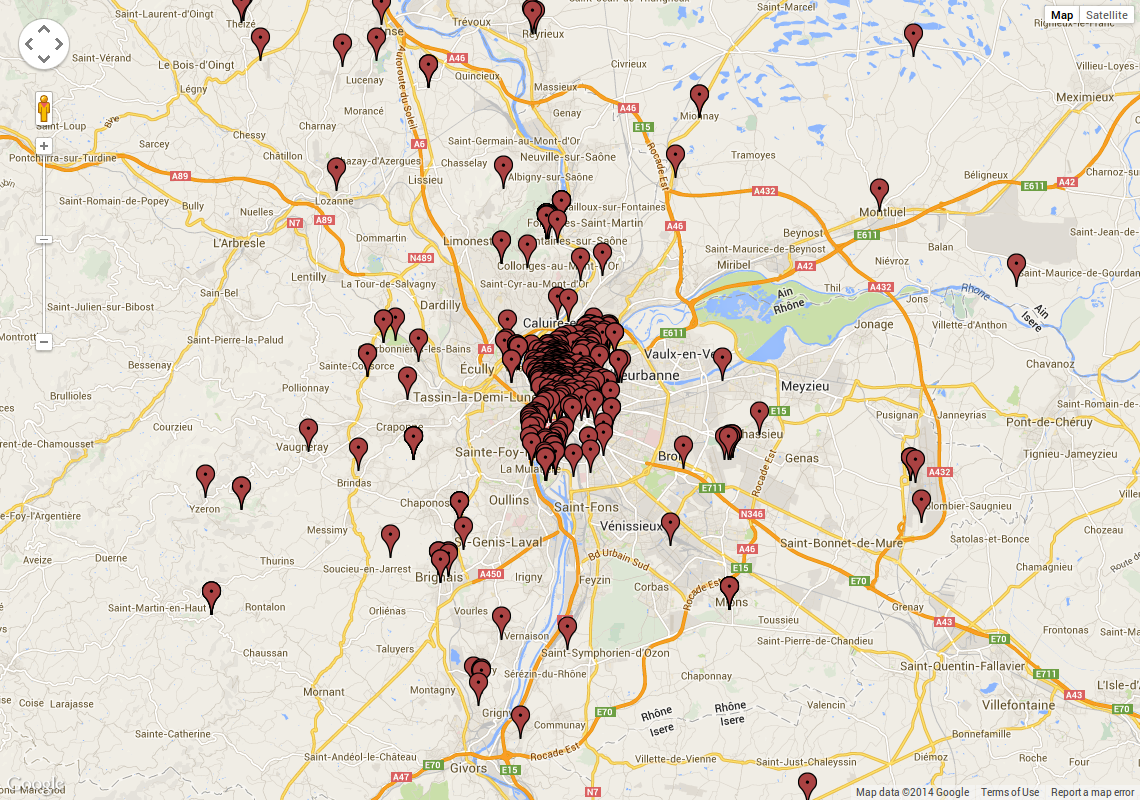
\includegraphics[width=14cm]{images/points.png}
    \caption{Affichage d'un échantillon des points}
    \label{fig:points}
\end{figure}

Cela nous donne déjà un premier aperçu. Nos points sont répartis autour de la ville de Lyon, et on constate une forte densité de points dans la ville.

Mais zoomons entre les deux fleuves de Lyon (figure \vref{fig:imprecision}).

\begin{figure}[!h]
    \centering
    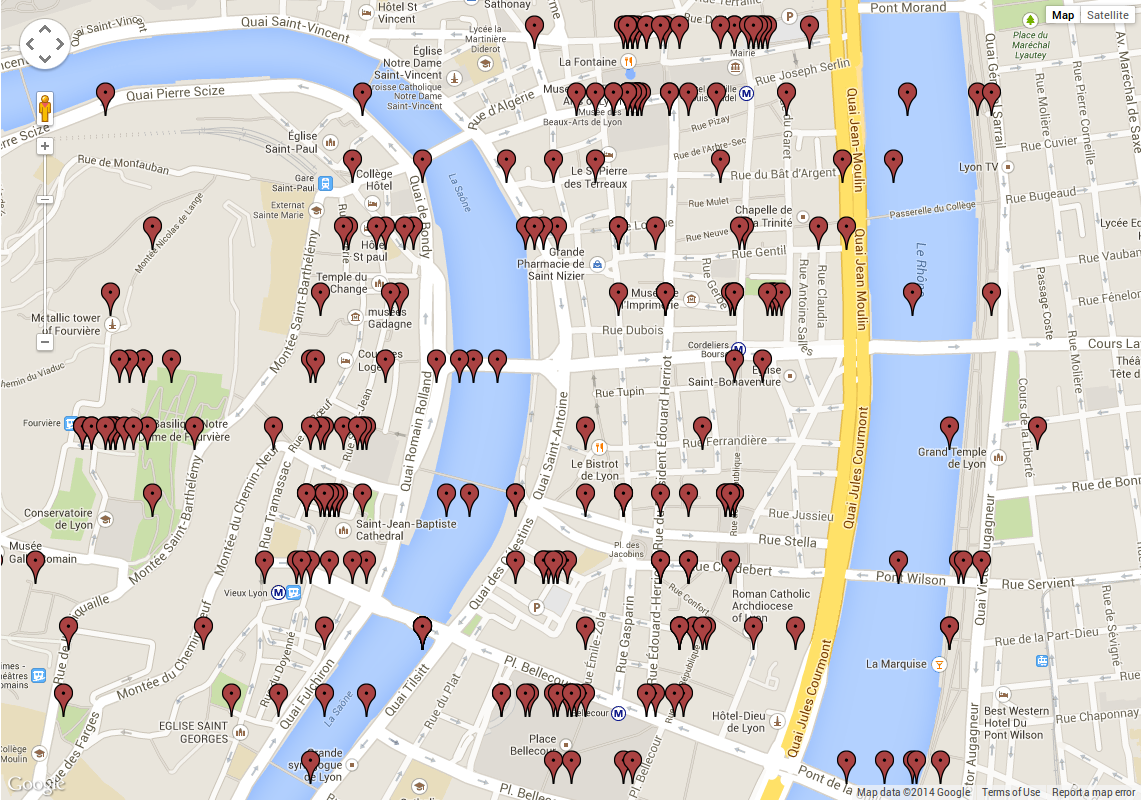
\includegraphics[width=14cm]{images/imprecision.png}
    \caption{Imprécision détectée lors du zoom}
    \label{fig:imprecision}
\end{figure}

On constate que tous les points se trouvent sur des lignes dont la séparation est très nette. Cela est dû à un manque de précision dans nos données de départ. Dans le fichier \textsc{csv} initial, nous remarquons en effet que les coordonnées GPS les plus précises que nous avons ne comportent que 4 chiffres après la virgule, ce qui explique la répartition étrange des points sur des lignes. Nous savons donc que cette erreur aura un impact sur la qualité de nos futurs clusters.


\section{Meanshift}

\section{TODO}
